\documentclass[draft=false]{oblivoir}
\author{Moon Il-chul \\ {icmoon@kaist.ac.kr}
   \and Shin Yongjin \\ {dreimer@postech.ac.kr} 
	\and Bae Hee-sun \\ {cat2507@kaist.ac.kr} }
\setcounter{chapter}{17}
\title{Chapter 17. Deep Generative Model}
\usepackage{kotex}
\usepackage{indentfirst}
\usepackage{graphicx}
\usepackage{hyperref}
\usepackage{amsmath}
\usepackage{amssymb}
\usepackage{amsfonts}
\usepackage{geometry}
\usepackage{algorithm}
\usepackage{algpseudocode}
\hypersetup{pdfborder={0 0 0}}
\renewcommand{\theequation}{\thechapter.\arabic{equation}}
\newlength\myindent
\setlength\myindent{5em}

\begin{document}

\maketitle
\tableofcontents

% 1. -----------------------------------------------------------------
\section{Taxonomy of Deep Generative Model}
4장의 Logistic Regression과 Naive Bayes Classifier를 비교할 때, 분류 모델(Discriminative Model)과 생성 모델(Generative Model)이라는 용어를 사용하였다. 최근에는 심층 생성 모델(Deep Generative Model)이 많이 발전함에 따라 분류 모델 뿐만 아니라 생성 모델에도 더 많은 관심이 모이고 있다.

심층 생성 모델은 기존의 생성 모델에서 심층 학습(Deep learning) 기법을 활용하는 모델을 일컫는다. 아래 그림(\ref{fig:17-1})과 같이 심층 생성 모델은 크게 명시적 분포 모델(Explicit Model)과 암묵적 모델(Implicit Model)로 나뉜다. 여기서 명시적과 암묵적이라는 단어가 수식하는 대상은 확률 분포이다. 명시적 모델이란 확률 분포의 모양에 대한 가정이 분명히 드러남과 동시에, 이 확률 분포에 대한 매개 변수(parameter)가 명확하게 드러나는 것이 특징인 모델이다. 예를 들어 어떤 모델이 정규 분포를 가정하고 평균과 분산을 명확히 밝힌다면 그 모델을 명시적 모델이라 부를 수 있다. 대표적으로 RBM(Restricted Boltzmann Machine)과 VAE(Variation Auto-encoder)가 있다. 이와 반대로 암묵적 모델이란 확률 분포를 가지기는 하나 그 확률 분포가 어떤 모양으로 어떤 매개 변수를 가지는지 명확히 드러나지 않는 경우를 말한다. 대표적으로 GAN(Generative Adversarial Network)이 있다.
\begin{figure}[ht] \centering
  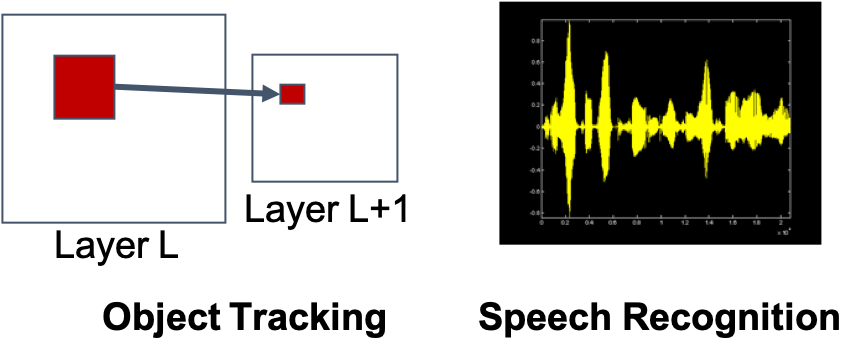
\includegraphics[scale=0.5]{fig1.png}
  \caption{Taxonomy of DGM}
  \label{fig:17-1}
\end{figure}
% 2. -----------------------------------------------------------------
\section{Explicit Deep Generative Model}

% 2.1 -----------------------------------------------------------------
\subsection{Overview}
명시적 심층 생성 모델(Explicit Deep Generative Model)의 계열에서는 추론(Inference) 단계에서 심층 학습 기법을 사용한다. 앞선 장에서 확률 그래프 모델에서 변분 추론(Variation Inference)이나 Gibbs Sampling과 같은 MCMC(Markov Chain Monte Carlo)기반의 추론을 학습하였다. 변분 추론은 최적화(Optimization) 과정을 통해 빠르게 학습을 할 수 있다는 장점이 있으나, 다양한 가정 속에서 근사치를 구할 수 밖에 없으며 수식 유도 과정이 복잡하다라는 단점이 있었다. 반면, 샘플링 기반의 추론은 학습 시간이 굉장히 길기 때문에 데이터가 많을 경우에는 학습이 어렵다라는 단점이 있다.

따라서 상기한 두 방법에서 존재하는 단점들을 극복하기 위해서 심층 학습 기법을 활용하여 추론을 진행하는 것이 명시적 모델이라고 할 수 있다.  예컨대 과거에는 수식을 통해서 정규 분포의 평균과 분산을 구했던 반면, 명시적 심층 생성 모델의 경우에서는 이를 뉴럴 네트워크(Neural Network)의 학습을 통해 얻을 수 있는 것이다. 본장에서는 대표적인 명시적 심층 생성 모델로 VAE(Variational Autoencoder)를 알아볼 것이다.

% 2.2 -----------------------------------------------------------------
\subsection{Autoencoders}
\begin{figure}[ht] \centering
  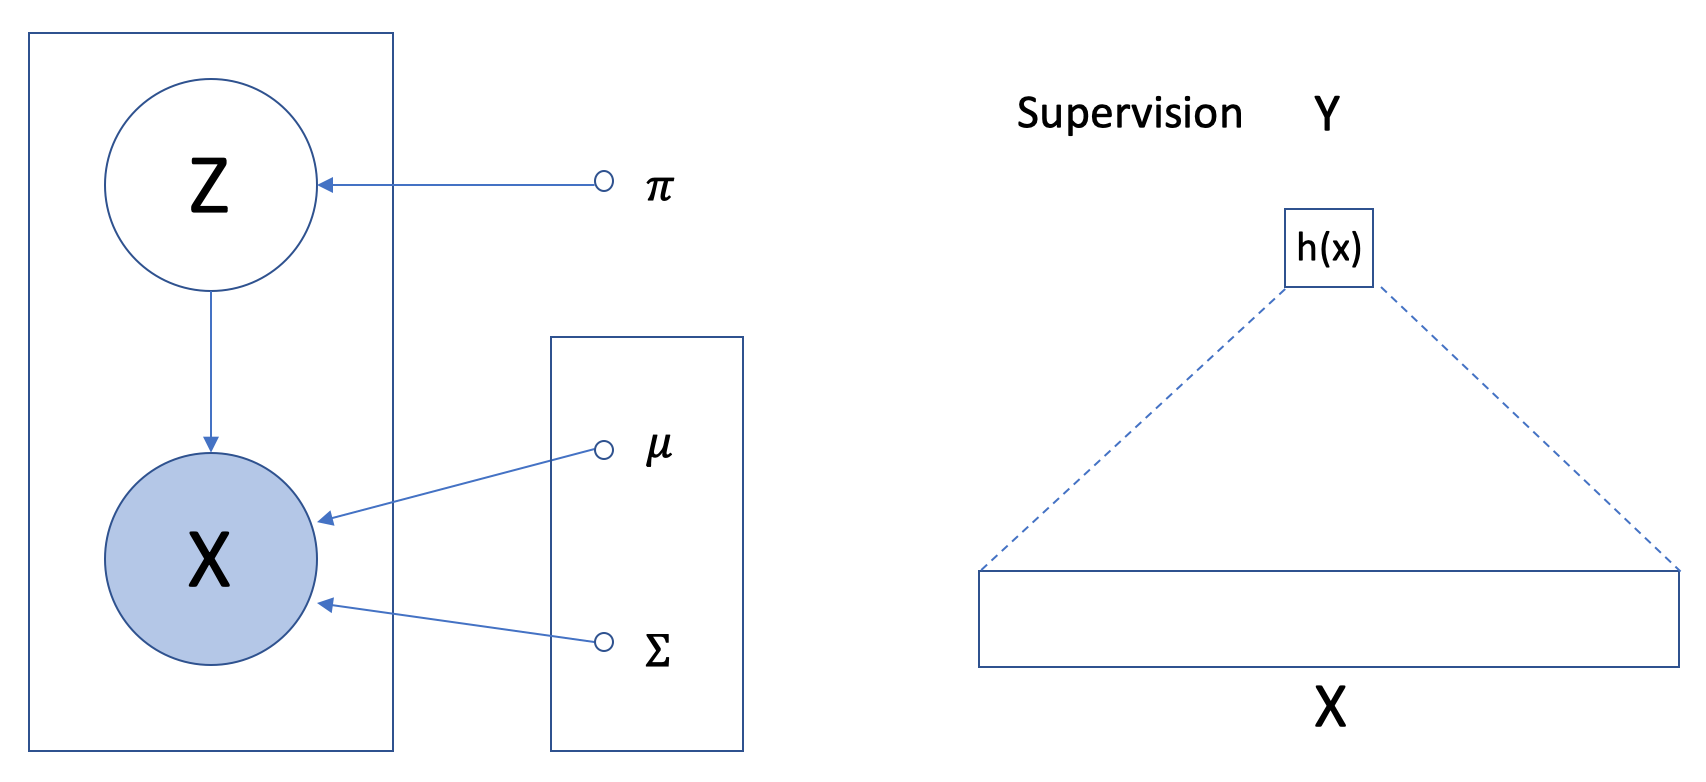
\includegraphics[scale=0.3]{fig2.png}
  \caption{GMM and Discriminative Model}
  \label{fig:17-2}
\end{figure}
VAE를 학습하기 이전에 오토인코더(Autoencoder)를 간략하게 살펴보도록 하겠다. GMM(Gaussian Mixture Model)은 대표적인 비지도 학습(Unsupervised Learning)의 예인데, 그림(\ref{fig:17-2})의 왼쪽과 같이 관측값인 $X$만을 이용하여 잠재 변수(Latent Variable) $Z$를 추론한다. 따라서 생성 모델 관점에서 이를 해석해본다면 $Z$를 알아내기만 한다면 $X$를 충분히 생성할 수 있다. 그러나 보통의 뉴럴 네트워크는 그림(\ref{fig:17-2})의 오른쪽과 같이 주어진 입력값($x$)에서 특정 값 $h(x)$을 얻어낼 수 있는 지도 학습(Supervised Learning)에 사용된다. 만약 그림(\ref{fig:17-2})에서 $h(x)$를 GMM의 잠재 변수 $Z$와 같이 주어진 입력값 $x$를 생성해낼 수 있는 잠재 정보로 사용할 수 있다면 뉴럴 네트워크를 통해서 충분히 GMM과 같은 모델을 구현할 수 있을 것이다. 이를 위해서는 단순히 $h(x)$를 얻어내는 것이 아니라 이를 이용해서 다시 $x$를 재현해내는 하나의 층이 더 필요하다. 이를 나타내면 아래 그림(\ref{fig:17-3})과 같다. 결과적으로 입력값 $x$를 통해 자기 자신과 유사한 $\hat{x}$을 재현해내는 것이 오토인코더(Autoencoder)라고 할 수 있다.
\begin{figure}[ht] \centering
  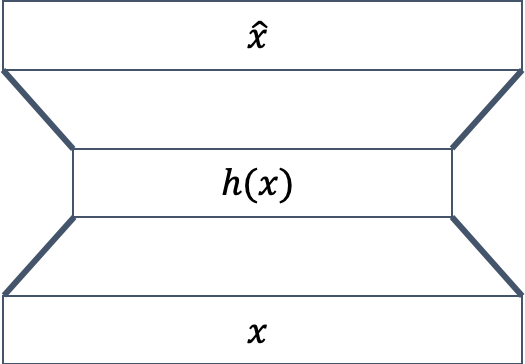
\includegraphics[scale=0.7]{fig3.png}
  \caption{Autoencoder}
  \label{fig:17-3}
\end{figure}
각 층은 어떤 구조의 뉴럴 네트워크로도 구성이 될 수 있으며 꼭 한 층일 필요도 없다. 만약 이러한 구조 안에서 Hidden Layer의 차원이 입력값(=출력값)의 차원과 동일하다면, 단지 단위 행렬(Identity Matrix)로 구성된 가장 간단한 오토인코더가 만들어질 수 있다. 그러나 만약 병목 구조(Bottleneck Structure)를 가지는 오토인코더일 경우 즉, Hidden Layer의 차원이 입력값(=출력값)의 차원보다 작아질 경우에는, GMM에서 잠재 변수가 입력값의 군집에 대한 정보만을 지니고 있었던 것과 같이 입력된 정보가 보다 축약된 정보의 형태를 지닐 수 있다. 전형적인 오토인코더의 구조는 다음과 같이 수식(\ref{eq:17-1})으로 나타낼 수 있다.
\begin{equation}
	\begin{split}
    \mathrm{Encoder} &: \quad h(x) = g(a(x)) = \sigma (W_{1}x + b_1)\\
	\mathrm{Decoder} &: \quad \hat{x} = f(\hat{a}(x)) = \sigma (W_{2}h(x) + b_2)
	\end{split}
	\label{eq:17-1}
\end{equation}
 이러한 개념은 압축 프로그램을 떠올리면 더욱 쉽게 받아들일 수 있을 것이다. 우리는 압축 프로그램을 사용할 때 압축을 푼 파일이 원본 파일과 완벽하게 동일할 것(lossless Compression)을 기대한다. 하지만 만약 우리가 특정 크기로 압축을 시키고 싶다고 요구를 한다면 압축을 풀었을 때 원본 파일과 완벽하게 일치하지 않을 것(lossy Compression)이라는 것을 독자들은 직관적으로 받아들일 수 있을 것이다. 이와 같이 오토인코더에서 $h(x)$로 차원이 축소됨에 따라 정보 손실(loss)이 일어날 수 밖에 없고 이를 다양한 손실 함수(Loss Function)를 통해 표현할 수 있다. 다음 수식(\ref{eq:17-2})의 $\mathcal{L}_{ce}$은 대표적인 손실함수인 크로스 엔트로피(Cross Entropy)를 나타낸다. 크로스 엔트로피는 Categorical Distribution을 비교할 때 주로 사용한다. 혹은 $\mathcal{L}_2$와 같이 제곱 오차(Squared Error)를 사용하여 연속한 값들을 가지는 분포를 비교해볼 수 있겠다.
 \begin{equation}
    \begin{split}
        \mathcal{L}_{ce} & = -\sum_{d=1}^{D}\big(x_{d}\log{(\hat{x}_d)} + (1-x_{d})\log{(1-\hat{x}_d)\big)}\\
 	\mathcal{L}_{2} & = \frac{1}{2}\sum_{d=1}^{D}(\hat{x}_d - x_d)^{2}
    \end{split}
    \label{eq:17-2}
 \end{equation}

 % 2.3 -----------------------------------------------------------------
\subsection{Stacked Denoising Autoencoders}
\begin{figure}[ht] \centering
  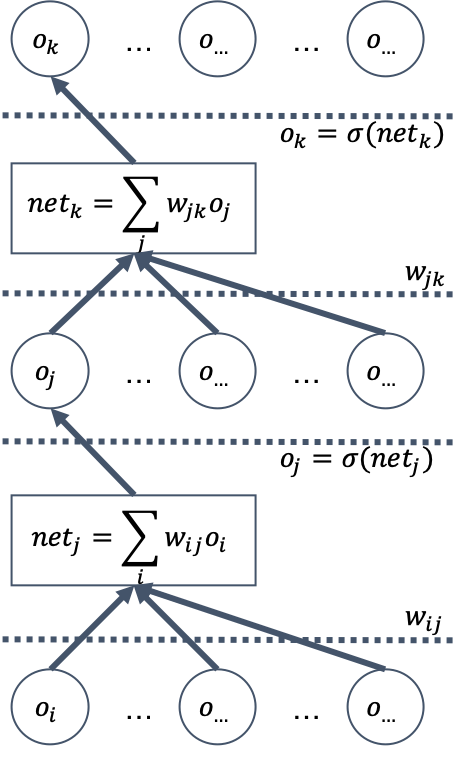
\includegraphics[scale=0.5]{fig4.png}
  \caption{Manifold of Dataset}
  \label{fig:17-4}
\end{figure}
이번 절에서는 기본 오토인코더 구조에서 노이즈(Noise)를 가미한 구조를 살펴보도록 하겠다. 구체적으로 이를 살펴보기 위해서는 수학적인 풀이가 필요하지만 그것은 책의 주제에서 벗어나므로 핵심 개념만 간단하게 살펴보면서 왜 이러한 구조가 발생하였는지를 짚어보도록 하겠다. 우선 우리가 보유한 데이터가 그림(\ref{fig:17-4})과 같은 선(위상 공간, manifold)으로 형성된다고 가정해보자. $x$는 선 위의 점이며, $x$에 임의의 노이즈를 가미하여 선 밖으로 나오게 된 지점을 $\tilde{x}$이라 하자.

만약 우리가 이를 관측하고자 할 때, 선 위에서 관측하는 것과 선 밖에서 관측하는 것 중 어느 것이 이 선을 더 잘 관찰할 수 있는 방법일까? 선을 잘 관찰하여 그것에 대한 설명을 할 수 있는 방법으로 접선을 이용하는 것이 있다. 무수히 많은 접선을 이용하면 관측한 선을 재현해낼 수 있기 때문이다. 따라서 본래의 질문으로 돌아간다면, 선 위 $x$에서 재현해낼 수 있는 접선은 해당 지점의 접선 밖에 없다. 그러나 $\tilde{x}$는 데이터가 이루는 선 위에 1개 이상의 수선을 내릴 수 있기 때문에 더 많은 접선을 만들어낼 수 있게 된다. 즉, 데이터 자체만으로 데이터가 내재하고 있는 다이나믹스(dynamics)를 파악하는 것보다 노이즈가 가미된 데이터($\tilde{X}$)을 통해 본래 데이터($X$)의 구조를 더 잘 파악할 수 있다라고 이해할 수 있겠다.

이렇게 노이즈를 가미한 데이터를 통해 잠재 변수를 더욱 잘 파악할 수 있는데 이를 오토인코더 구조로 표현을 하자면 아래 그림(\ref{fig:17-5})와 같다.
 \begin{figure}[ht] \centering
  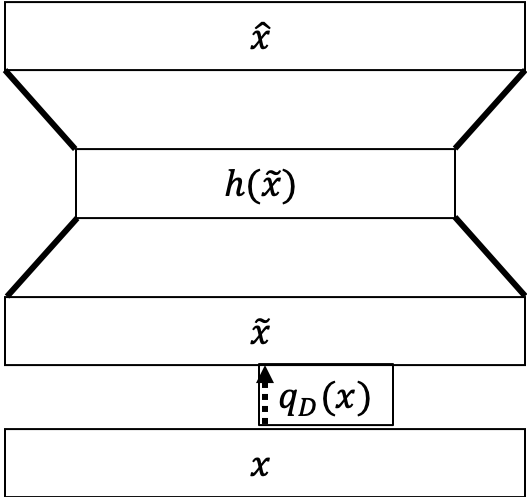
\includegraphics[scale=0.5]{fig5.png}
  \caption{Stacked Denoising Autoencoders}
  \label{fig:17-5}
\end{figure}
만약 해당 모델이 노이즈에 민감한 모델이라면, 즉 노이즈가 변할 때마다 값의 변동폭이 큰 모델이라면, 이 모델을 통해 얻게 된 잠재 변수의 값을 활용하기 어려울 것이다. 따라서 위의 그림(\ref{fig:17-5})과 같은 오토인코더를 Denoising Autoencoder라 부르는데 이는 임의로 가미된 노이즈를 포함하는 데이터(Noised Input)가 입력됨에도 불구하고 그 노이즈를 없애면서(Denoise) 실제 데이터(Clean Output)를 재현해낼 수 있기 때문이다. 수식(\ref{eq:17-1})과 유사하게 이를 나타내어 본다면 다음(\ref{eq:17-3})과 같다.
\begin{equation}
	\begin{split}
      \mathrm{Encoder} &: \quad h(\tilde{x}) = g(a(x)) = \sigma (b_1 + W_{1}\tilde{x})\\
      \mathrm{Decoder} &: \quad \hat{x} = o(\hat{a}(\tilde{x})) = \sigma (b_2 + W_{2}h(\tilde{x}))\\
      \mathrm{Noise Process} &: \quad \tilde{x} = q_{D}(x)
	\end{split}
	\label{eq:17-3}
\end{equation}
$q_{D}$함수에 대한 정의는 상황에 따라 달라질 수 있다. 연속형 변수의 경우, 가우시안 노이즈(Gaussian Noise)를 가미할 수 있다. Categorical 분포를 따를 경우에는 마스킹 노이즈(Masking Noise)를 가미할 수 있다. 손실 함수는 위에서 언급한 수식 (\ref{eq:17-2})을 동일하게 사용할 수 있는데, 이 때 주의할 점은 손실 함수에서 $\tilde{x}$는 사용되지 않는다는 점이다.
\begin{equation}
	\begin{split}
		\mathrm{Gaussian Noise} &: \quad q_{D}(x) = x+\epsilon, \epsilon \sim \mathcal{N}(\mu_{D}, \Sigma_{D})\\
        \mathrm{Masking Noise} &: \quad q_{D}(x) = x+\epsilon, \epsilon \sim Bernoulli(p)\\
	\end{split}
    \label{eq:17-4}
\end{equation}
Stacked Denoising Autoencoder에서 무작위성(Randomness)이 포함되기 시작했다. 이 무작위성은 $q_D$ 함수에서 가우시안이나 베르누이 분포에서 샘플링을 하여 노이즈를 생성할 때 발생한다. 이러한 노이즈가 전체 모델의 회복탄력성(Resilience)을 만들어주는 요소로 작용하는데, 이것이 필요한 이유는 앞서 설명하였듯이 작은 변화로 인해 결과가 너무 급격하게 바뀌지 않는 모델을 만들고 싶기 때문이다. 그러나 Stacked Denoising Autoencoder의 구조에서는 무작위성이 오로지 $x$에만 부여되기 때문에 Batch Process가 완료된 시점 이후에는 무작위성의 영향은 없다. 왜냐하면 매개 변수의 학습이 끝난 이후에는 뉴럴 네트워크는 오직 Deterministic한 구조이기 때문이다. 이러한 문제점을 해결하기 위해 발전된 모델이 바로 Variational Autoencoder라고 할 수 있겠다.

 % 2.4 -----------------------------------------------------------------
\subsection{Detour: Inference with Latent Variables}
잠재 변수에 대한 추론은 왜 어려울까? 이전에 학습한 내용이지만 간단하게 복습을 해보도록 하겠다. $X$는 관측된 변수이고 $Z$는 잠재 변수이며, 두 변수 모두 확률 변수(Random Variable)이라 가정한다. 이 경우에 확률 변수의 확률 분포에 상응하는 매개 변수 $\theta$가 필요해진다. 1장에서 사용한 압정던지기 예시를 다시 사용해보겠다. 앞정을 던졌을 때 앞면 혹은 뒷면이 나올 확률은 정해져 있다. 즉, 우리가 흔히 마주하는 문제는 파라미터 $\theta$가 전제되어 있는 상황이라고 할 수 있다. 이 때 궁금한 것은 $X$를 볼 수 있는 상황이 얼마나 되는가이다. 다시 말해, $P(X|\theta)$를 구해야 하는 문제가 된다. 그러나 만약 $Z$까지 존재하는 상황이라면 이는 다음과 같은 수식(\ref{eq:17-5})으로 표현한다.
\begin{equation}
	\begin{split}
	P(X|\theta) & = \sum_{Z} P(X,Z|\theta) \\
    \ln{P(X|\theta)} & = \ln{(\sum_{Z} P(X,Z|\theta))}
	\end{split}
	\label{eq:17-5}
\end{equation}
$X$와 $Z$의 결합 확률 분포(Joint Distribution)을 만들어야 하는 상황에서 $Z$는 우리가 모르는 값이므로 Marginalize out하여 표현을 할 수 있게 된다. P라는 확률 분포가 지수 함수의 형태를 띄기 쉬우므로, 추후에 있을 최적화 과정의 계산상의 편의를 위해 $log$를 씌어주게 된다. 이때 우리가 잘 알고 있는 Gradient Descent/Ascent를 계산하는 순간 $log$ 속에 있던 값들은 분모로 내려가면서 $\frac{\frac{\partial}{\partial X} \sum_{Z}P(X,Z|\theta)}{\sum_{Z}P(X,Z|\theta)}$와 같이 나타난다. 따라서 이 수식들은 간략하게 나타내기가 힘들어지므로 직접적으로 추론을 하기가 어렵게 된다. 뿐만 아니라, $Z$의 차원이 어느 정도인지 모르기 때문에 무한대에 가까워질 수도 있다. 이렇게 $Z$를 다루기 어려운 상황(Intractable)을 해결하기 위해서 $\ln{P(X|\theta)}$의 ELBO(Evidence Lower Bound)를 구하여 근사치를 구하려는 시도를 한다.

 % 2.5 -----------------------------------------------------------------
\subsection{Detour: Evidence Lower bound}
ELBO를 유도하는 과정을 간략하게 되짚어 보겠다. 여기에서 사용하는 표기는 이전 강의의 표기와 동일하게 유지한다. 따라서 $E$는 관측값(Evidence)를 뜻하고, $H$는 잠재 변수(Hidden Variable)을 나타낸다. 그리고 $Q$라는 임의의 확률 분포를 도입하는데, 이 분포는 우리가 잘 받아들일 수 있는 분포이거나 Mean Field 가정을 할 수 있는 분포를 차용한다.
\begin{equation}
	\ln{P(E)} = \ln{\sum_{H}P(H,E)} = \ln{\sum_{H}Q(H)\frac{P(H,E)}{Q(H)}}
	\label{eq:17-6}
\end{equation}
위의 수식(\ref{eq:17-6})을 더 이상 전개하는 것은 불가능하지만 $log$함수가 볼록(Concave) 함수이기 때문에 얀센 부등식(Jensen's Inequality)를 활용할 수 있다. 따라서 다음과 같이 수식을 변형할 수 있다.
\begin{equation}
	\begin{split}
		\ln{\sum_{H}Q(H)\frac{P(H, E)}{Q(H)}}
        & \geq \sum_{H}Q(H)\ln{\frac{P(H,E)}{Q(H)}} = \mathrm{ELBO}\\
        & = \sum_{H}Q(H)\ln{P(H,E)} - Q(H)\ln{Q(H)}\\
        & = \sum_{H}Q(H)\big( \ln{P(E)} + \ln{P(H|E)}\big) - Q(H)\ln{Q(H)}\\
        & = \sum_{H}Q(H)\ln{P(E)} - Q(H)\ln{\frac{Q(H)}{P(H|E)}}\\
        & = E_{Q(H)}\ln{P(E|H)} - D_{KL}(Q(H) || P(H|E))
	\end{split}
	\label{eq:17-7}
\end{equation}
위 수식(\ref{eq:17-7})의 마지막 줄은 극히 중요하므로, 독자들은 이 형태를 반드시 기억하기를 바란다.

모델의 매개 변수 $\theta$와 확률 분포 $Q$의 매개 변수 $\lambda$를 통해 다음(\ref{eq:17-8})과 같이 ELBO를 나타낼 수 있다.
\begin{equation}
	\mathcal{L}(\lambda, \theta) = \sum_{H}Q(H; \lambda)\ln{P(E|H,\theta)} - Q(H; \lambda) \ln{Q(H; \lambda)}
	\label{eq:17-8}
\end{equation}
KL divergence가 0 이상의 값만을 가지므로, 독자들은 ELBO를 최대화하는 방향은 KL-Divergence인 $D_{KL}[Q(H; \lambda)||P(H|E,\theta)]$가 0에 최대한 가까워지는 방향이라는 것을 알 수 있을 것이다. 즉, $Q(H; \lambda) = P(H|E, \theta)$를 만족하도록 $\lambda$를 통해 $Q$를 변형시켜나간다 (Maximization). 그리고 $Q$가 변하면 자연스럽게 ELBO도 변하기 때문에 다시금 ELBO를 최대화 할 수 있도록 계산이 필요하다 (Expectation).

% 2.6 -----------------------------------------------------------------
\subsection{Detour: Amortized Analysis and Inference}
분할상환분석(Amortized Analysis)에 대해서 엄밀하게 다루는 것은 본 교재의 학습 범위에서 벗어나므로 간략하게 이에 관한 개념만을 언급하면서 어떻게 VAE와 연결이 되는지를 알아보도록 하겠다.

데이터 구조 중 하나인 해시 테이블(Hash Table)을 예로 살펴보자. 해시 테이블에서 하나의 데이터를 추가(Insert)할 때 걸리는 시간이 $O(1)$ (order of constant)이라고 배운다. 그러나 해시 테이블이 꽉 차있는 경우에는 $O(N)$ (order of N)으로 증가한다. 즉, 데이터가 어떤 순서에 있느냐에 따라 $O(1)$이 될 수도 있고 $O(N)$이 될 수도 있다. 그렇다면 해시 테이블에서 데이터를 추가할 때 $O(1)$이라고 단지 암기하는 게 옳다고 할 수 있을까? 우리가 실제 연산(Operation) 시간을 구하기 위해서는 직접 데이터를 가지고 실험을 해볼 수 밖에 없다. 따라서 데이터의 사이즈와 순서(Sequence)가 어떻게 될지에 대한 가정을 기반으로 계산 복잡도 분석(Complexity Analysis)를 하는 것이 바로 분할상환분석이다.

위의 개념을 확률 그래프 모델로 가져와보도록 하자. 이전까지 우리가 학습해온 MCMC나 변분 추론(Variational Inference)은 사람이 직접 수식을 유도하여 모델링을 하고 난 이후에 데이터를 넣어 학습을 시켰다. 그러나 분할상환추론(Amortized Inference)은 실제 데이터를 먼저 넣어서 근사 함수를 유도하도록 하는 것이 핵심 개념이다. 변분 추론에서 잠깐 언급하였던 Black Box Variational Inference에서 더욱 나아가서 보다 유연한 구조로 학습이 가능한 뉴럴 네트워크를 통해 이러한 분할상환추론이 가능하게 되었다. 예를 들어, 관측치(Evidence)가 주어졌을 때, 가우시안 분포를 만들어내기 위해 필요한 매개 변수인 평균($\mu = f(E)$)과 분산($\Sigma = g(E)$)을 도출해낼 수 있는 뉴럴 네트워크 $f, g$를 만드는 셈이다.

% 2.7 -----------------------------------------------------------------
\subsection{Detour: Amortized Inference}
기본적인 확률적 그래픽 모델(probabilistic graphical model)는 다음(\ref{eq:17-9})과 같이 표현된다.
\begin{equation}
	P(H,E) = P(E|H) \prod_i P(H_i|H_Parent(H_i))
	\label{eq:17-9}
\end{equation}
변분 추론에서는 $P(H|E, \lambda)$에서 P라는 posterior 확률 분포 함수를 직접 근사하는 대신, 복잡하지 않은 확률 분포와 추가적인 변분 인자인 $\phi$를 가지는 $q_E(H;\phi)$를 만들 것이다. $q_E(H;\phi)$의 일반적인 형태로 mean field assumption을 만족하는 것을 가정한다. 즉, $q^{MF}_{E}(H; \phi) = \prod_{i} q(H_i;\phi_i)$가 성립한다. $\phi$를 업데이트하여서 KL divergence를 optimize하고 확률 분포 함수$P$를 근사하도록 한다. 기존의 변분 추론은 앞서 언급하였던 바와 같이 매개 변수 $\phi$에 대해서 수식을 유도한 다음 모델 학습을 시작한다. 반면에 분할상환추론은 이렇게 추론에 관여하는 수식에 대한 직접적인 유도 없이도 뉴럴 네트워크를 데이터(E)를 통해 학습을 해서 추론에 관여하는 함수를 근사하겠다라는 것(\ref{eq:17-10})을 의미한다. 이렇게 학습할 경우, $q(H|E;\phi)$과 $P(H|E,\lambda)$의 KL divergence를 최소화하게 된다.
\begin{equation}
	q^{MF}(H|E;\phi) = \prod_i q(H_i; NN_i (E,\phi_i))
	\label{eq:17-10}
\end{equation}
% 2.8 -----------------------------------------------------------------
\subsection{ELBO and Variational Autoencoder}
VAE이란  확률적 오토인코더(probabilistic autoencoder)이다. Stacked Denoised Autoencoder는 오직 Batch Process에서만 무작위성이 작용하기 때문에 우리가 원하는 모델이 아니라고 언급한 바가 있다. 우리가 실제로 원하는 확률적 오토인코더란 $h(x)$가 확률 변수가 되는 모델이다. 확률 변수가 존재하기 위해서는 확률 분포가 존재하고 이에 상응하는 매개 변수가 존재하는 것을 말한다. 따라서 확률 분포와 매개 변수를 정의할 수 있도록 $h(x)$를 만들어줘야 한다. 이런 상황 아래에서 다시 ELBO를 떠올려 보자(\ref{eq:17-11}).
\begin{equation}
	\mathcal{L} = -D_{KL}\Big(q_{\phi}(H|E)||p_{\theta}(H)\Big)
    + \mathbb{E}_{q_{\phi}(H|E)}[\log{p_{\theta}(E|H)}]
    \label{eq:17-11}
\end{equation}
$q_{\phi}(H|E)$는 $E$가 주어졌을 때 $H$에 관한 확률 분포 함수이다. 따라서 관측치 $E$를 넣으면 잠재 변수(Latent Variable)인 $H$가 도출된다. 반면에 $p_{\theta}(E|H)$는 $H$가 주어졌을 때 $E$에 관한 확률 분포 함수이다. 그러므로 잠재 변수 $H$를 넣으면 $E$를 도출하게 된다. 이러한 이유로 앞쪽의 KL divergence의 부분은 Encoder, 뒤쪽은 기대값 부분은 Decoder로써 역할을 할 수 있겠다. 즉, ELBO 자체만으로도 오토인코더의 역할을 할 수 있게 된다(그림\ref{fig:17-6}). 다만, 이것만으로 우리가 원하는 오토인코더의 역할을 하는 모델을 얻기는 쉽지 않다. 앞서 언급하였듯이 확률 분포의 매개 변수를 어떻게 만들어주는가에 대한 해답이 제시되어야만 모델을 얻었다고 할 수 있을 것이다.
\begin{figure}[ht] \centering
  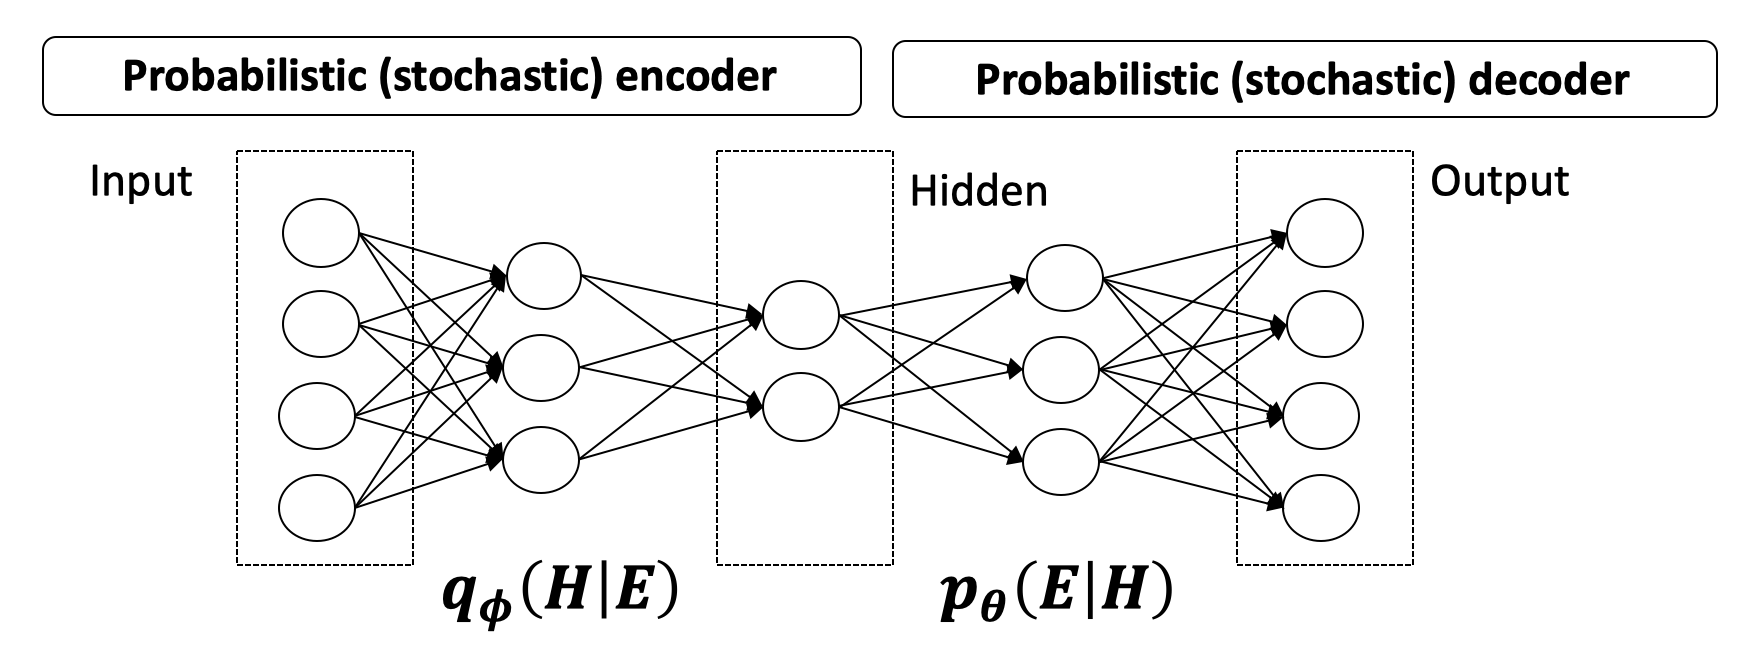
\includegraphics[scale=0.5]{fig6.png}
  \caption{ELBO = Encdoer + Decoder}
  \label{fig:17-6}
\end{figure}

한가지 짚고 넘어갈 점은  KL divergence는 사전 확률(Prior Probability)인 $p$ 확률 분포와 연관이 있다는 것이다. 즉, 인코딩을 진행하는 $q$ 확률 분포는 사전 확률 $p$와 크게 차이가 없게 만들어져야 하는 것을 의미하므로 정규화(Regularization)의 역할을 한다고 볼 수 있다. $q$에 의해서 관측값 $E$가 사전 확률과 크게 다르게 인코딩이 되어버린다면  KL divergence의 값이 커져버릴 수 밖에 없다. 따라서 인코딩은 사전 확률에 의해 제약을 받으면서 학습이 이루어진다. 반면 ELBO가 증가하기 위해서는 로그우도(Log likelihood)의 기대값(Expectation)이 증가해야만 하므로, 앞서 인코딩된 $H$가 $E$로 최대한 복원(Reconstruct)이 잘 되도록 이루어져야만 한다. 다만, 앞서 언급하였듯이 사전 확률에서는 너무 많이 벗어나지 않도록 정의된다.

% 2.9 -----------------------------------------------------------------
\subsection{Variational Autoencoder}

\begin{figure}[ht] \centering
  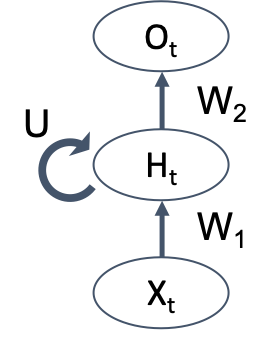
\includegraphics[scale=0.7]{fig7.png}
  \caption{VAE}
  \label{fig:17-7}
\end{figure}

변분 추론에서 $q$분포는 $p$분포가 복잡하기 때문에 이를 근사하기 위해 도입된 분포이다. 따라서 Mean field Variational Inference와 같이 팩토리얼(Factorial) 형태로 $q$분포를 표현하거나 혹은 켤레사전분포(Conjugate Prior Distribution)을 통해 수식 유도를 조금 간단하게 만들 수 있었다. 그러나 VAE에서는 Mean Field 가정은 굳이 하지 않아도 되지만, 잠재 변수에서는 연속형이라는 가정이 포함되어야 한다. (물론, 다양한 연구가 지속되면서 연속형이라는 가정이 더 이상 포함되지 않아도 되지만 그럼에도 불구하고 초기의 VAE에서는 연속형이라는 가정이 존재하였다.) 기존의 확률 그래프 모델에서 변분 추론을 다룰 때에는 DAG(Directed Acyclic Graph)으로 실선만 존재하였다. 그러나 VAE가 도입되면서 복원과정(Reconstruct)에 해당하는 Decoder에 덧붙여 추론과정(Inference or Recognition)에 해당하는 Encoder를 포함시키기 위해서 역방향의 붉은 색 점선이 도입되었다.

이러한 VAE는 많은 기계 학습 문제들에서 아주 일반적인 매개 변수 학습 과정이라고 할 수 있겠다. 따라서 VAE를 통해 매개 변수에 대해서 별다른 수식 유도 과정이 없이도 효율적으로 근사치를 구해볼 수 있게 되었다. 뿐만 아니라 사후 확률 추론에 대해서도 효율적인 방법이라 할 수도 있다. 그리고 이전에는 학습을 할 때 전체 데이터에 대한 Gradient를 계산하고 확률 분포를 계산하는 업데이트 과정이 있었던 반면, VAE에 들어와서는 데이터 하나씩 주입하여 Encoder 네트워크와 Decoder 네트워크에 대한 학습이 가능하게 되었다. 따라서 관측 데이터 하나가 들어감에 따라 잠재 변수가 어떻게 학습이 되는지를 관측할 수 있다.

% 2.10 -----------------------------------------------------------------
\subsection{Objective function of Variational Autoencoder}
앞 단원에서 variational autoencoder(VAE)의 구조에 대해 알아보았으므로, 실제로 어떻게 학습하는지 목적함수에 대해 알아볼 것이다. VAE의 목적함수는 ELBO로부터 쉽게 유도할 수 있다. 앞에서도 언급했다시피 ELBO는 $E_{q_\phi(z|x)} [logp_\theta (x|z)]-D_{KL} \Big(q_\phi (z|x)||p_\theta (z)\Big)$이며, 앞부분은 decoder 역할을, 뒷부분은 encoder 역할을 한다. 뒷부분은 z의 prior 확률 분포 또한 언급하므로 사전정보를 넣는 역할과, q 분포의 regularizer의 역할도 하고 있다. 이것이 기본적인 손실함수다.

여기서 문제가 하나 발생한다. VAE가 도입된 것은 잠재변수에 무작위성을 부여하기 위함이었다. 실제로 VAE에서는 확률분포를 이용해서 잠재변수를 표현하기 때문에 잠재변수가 random variable이 된다. 그러나 기본적으로 신경망 구조는 deterministic한데, 이것은 신경망 구조의 값들을 계산할 때 deterministic variable의 경사를 계산해서 back propagation하기 때문이다. 이것을 해결하기 위해 Reparameterization trick이나 Stochastic Gradient Variational Bayes 등을 사용한다.

특별히 Reparameterization Trick에 대해 더 알아보겠다. 잠재변수 $\tilde{z}$에 대해서 $\tilde{z}\sim q_\phi (z|x)$는 확률분포이므로 랜덤 변수 z가 어디에서 추출되는지를 말해주는데, 해당 확률분포에는 변하지 않는 임의의 값이 반드시 있을 것이다. (가령, 정규분포의 경우 평균과 표준편차를 가진다.) 이것은 결정된 인자이다. 이 인자들로 이루어진 미분가능한 함수 $g_\phi$를 정의한다면, 랜덤변수 $\tilde{z}$ 는 정해진 값 $g_\phi (\epsilon, x)$ 와 난수 $\epsilon \sim p(\epsilon)$의 조합으로 생각할 수 있을 것이다. 이 때 z의 randomness는 $\epsilon$에서 발생하는 것이다. noise에 대한 샘플링이 필요한 것은 어쩔 수 없다. 다만 noise 범위가 주어져 있다는 가정하에서는 deterministic한 할당을 하겠다는 것이 함수$q_\phi$와 함수$g_\phi$의 차이이다.

$q_\phi$를 모델하기 위해서 분할상환추론를 수행할 것이다. 적용하면 $q_E (H;\phi)$ 대신에 $q(H|E;\phi) = \prod_i q(H_i; NN_i (E;\phi_i))$가 된다. 만약 q 확률분포를 정규분포라고 가정한다면, 즉, $q_\phi (z|x)\sim N(\mu(x;\phi), \Sigma(x;\phi))$라면 다음(\ref{eq:17-12})과 같이 정리할 수 있다.
\begin{equation}
	\begin{split}
	g_\phi (\epsilon, x) &= \mu(x;\phi) + e\sqrt{\Sigma(x;\phi)}, e\sim N(0,1) \\
	\mu_i(x; \phi) &= NN_{i}^{\mu}(x|E;\phi^{\mu}_i), \Sigma_i (x;\phi) = NN_{i}^{\Sigma} (x|E;\phi_{i}^{\Sigma}) 
	\end{split}
	\label{eq:17-12}
\end{equation}
잠재변수를 추출하는 데 있어 확률분포 $q_\phi$를 이용할 경우에는 해당 분포의 전체 치역에 대한 경사를 계산하는 데 비해 $\epsilon$에만 randomness를 부여할 경우에는 (0,1)의 범위에 대해서만 경사를 계산하게 되고, 따라서 back propagation에 의한 차이는 줄어들지만 $\mu$과 $\sigma$를 그대로 사용할 수 있다는 장점이 있다. 만약 확률분포로 정규분포를 선택하지 않는다면 reparameterizaion 수식을 바꿔서 다른 인자를 추론하면 된다.

다시 ELBO에서 decoder 부분의 Loss를 생각해보자. $E_{q_\phi(z|x)} [f(z)]$를 z에 대하여 reparameterization하면 $E_{p(\epsilon)} \Big[f\Big(g_\phi(\epsilon,x)\Big)\Big]$로 표현할 수 있다. $E_{p(\epsilon)} \Big[f\Big(g_\phi(\epsilon,x)\Big)\Big]$는 $p(\epsilon)$에 대한 평균이므로 이는 곧 $\frac{1}{D}\sum_{d=1}^{D}f\Big(g_\phi (\epsilon^{(d)},x)\Big)$와 같다(단 $\epsilon^{(d)}\sim p(\epsilon)$).

이것을 ELBO에 적용하면 $\tilde{\mathcal{L}} = \frac{1}{D}\sum_{d=1}^{D}(logp_\theta (x|z^{(d)})) - D_{KL}\Big(q_\phi (z|x)\Vert p_\theta (z)\Big) $이다. $z^{(d)}$는 개별 데이터 마다 $z^{(d)} = g_\phi (\epsilon^{(d)}, x)$를 따르며, $\epsilon^{(d)}\sim p(\epsilon) $이다. KL Divergence 역시 Monte Carlo 방법으로 어렵지 않게 구할 수 있으므로, 이제 Monte Carlo방법으로 ELBO를 계산할 수 있다. VAE의 손실함수를 정의하였으므로 다음 단원에서는 결과를 알아볼 것이다.

% 2.11 -----------------------------------------------------------------
\subsection{Reparameterization Trick}
VAE의 손실함수에 대해 알아보았는데, 손실함수를 만드는 데에 핵심적인 역할을 한 것이 Reparameterization trick이었다. 이 단원에서는 reparameterization에 대해 시각화하여 다루겠다.

Reparameterization이란 미지의 확률분포를 정해진 값과 알 수 있는 확률분포의 조합으로 변환하는 trick인데, 이 때 확률분포의 기대값이 일치해야 한다. 예를 들어 VAE에서는 reparameterization을 ELBO의 decoder 부분을 이해할 때 사용하는데, 수식(\ref{eq:17-13})과 같다,
\begin{equation}
	E_{q_\phi(Z|X)}\Big[f(z) \Big] = E_{p(\epsilon)}\Big[f\Big(g_\phi(\epsilon, x) \Big) \Big]
	\approx \frac{1}{L} \sum_{l=1}^L f\Big(g_\phi (\epsilon^{(l)}, x) \Big)
	\label{eq:17-13}
\end{equation}
수식(\ref{eq:17-13})에서 $q_\phi(Z|X)$는 미지의 확률분포이므로 알려진 것이 없다. 이것을 그대로 모델링에 이용하기에는 어려움이 있으므로, 표준정규분포와 같은 분포로 바꿔줄 것이다. 이 때 등호의 왼쪽과 오른쪽에 있는 각각의 기대값은 같아야 한다. 이를 고려하여 deterministic하고 미분 가능한 $g_\phi$ 함수를 정의한다. $\epsilon^{(l)}$은 각 데이터마다 있는 에러이며, $g_\phi (\epsilon^{(l)}, x)$에서 나오는 변수와 $q_\phi(Z|X)$에서 만들어지는 변수가 같도록 g를 정의해야 한다. 랜덤한 부분을 없애는 이유는 back-propagation을 하기 위함이다. 

\begin{figure}[ht] \centering
  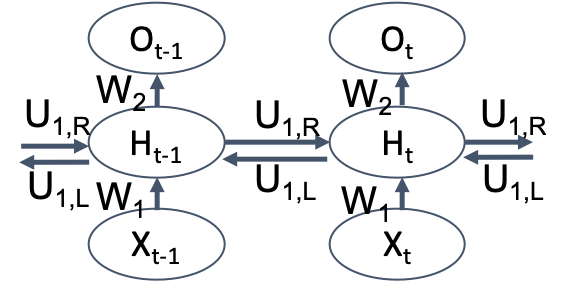
\includegraphics[scale=1]{fig8.png}
  \caption{Structure of Reparameterization}
  \label{fig:17-8}
\end{figure}

그림 (\ref{fig:17-8})을 보면 reparameterization이 무엇인지 시각화되어 있다. 왼쪽 그림의 경우, back propagation하여 구해야 하는 변수 z 자체가 stochastic한 반면에 오른쪽 그림의 경우에는 stochastic한 부분을 $\epsilon$이라는 에러 변수로 분리하였다. back propagation을 한다면 왼쪽 그림은 z가 크게 변하여 좋지 않은 것에 비해 오른쪽 그림은 정해진 인자로 쓸 수 있는 평균, 분산과 같은 부분만 모델링하여 정하므로 의미가 있다. reparameterization은 이러한 역할을 한다.

% 2.12 -----------------------------------------------------------------
\subsection{Neural Network Structure of VAE}

\begin{figure}[ht] \centering
  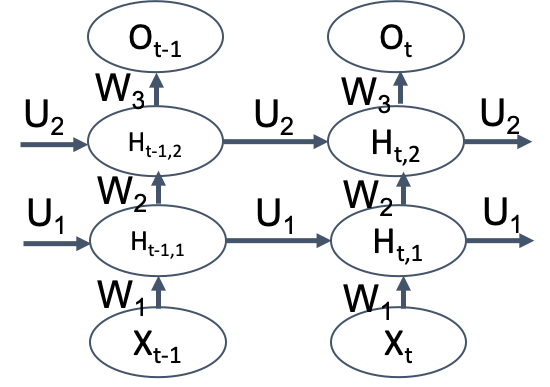
\includegraphics[scale=1.1]{fig9.png}
  \caption{VAE as Neural Net}
  \label{fig:17-9}
\end{figure}

이번 단원에서는 신경망 구조를 이용하여 VAE를 학습할 것이다, 전통적인 Autoencoder 구조의 문제는 잠재변수 z가 deterministic히다는 것이었고, 이것을 해결하기 위해 확률 분포로부터 잠재변수 z를 생성해내어 잠재변수에 stochastic한 성질을 부여해 주었다. 그러나 stochastic한 잠재변수를 back propagation으로 학습하기에는 어려움이 있다는 문제가 나타났고, 그러므로 VAE를 신경망 구조로 학습하려면 앞에서 배운 Reparameterization trick을 적용하여 잠재변수의 deterministic한 부분을 학습해야 한다(잠재변수가 정규분포를 따른다면 $\mu$와 $\sigma$를 학습하는 것에 해당한다). 다시 말해 신경망 구조의 역할은 deterministic한 인자를 알기 위한 weight들을 학습하는 것이 되겠다.

일반적인 AE(autoencoder)와의 차이는 z가 아닌 $\mu$와 $\sigma$에 대한 back propagation을 실행한다는 것이다. 그 외에는 다른 AE와 동일하다.

\begin{figure}[ht] \centering
  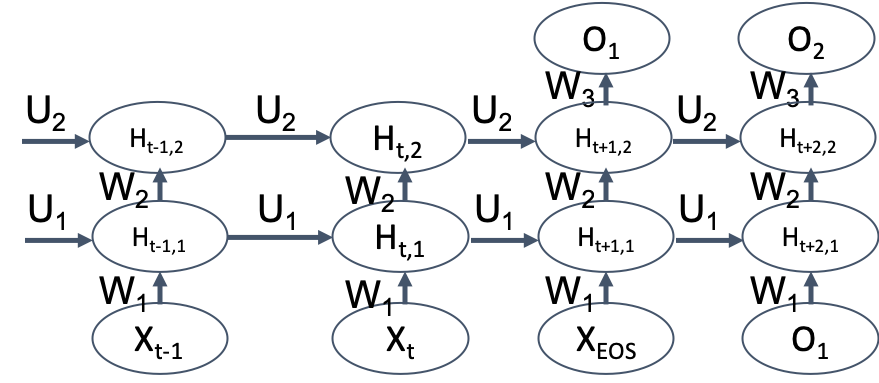
\includegraphics[scale=1.8]{fig10.png}
  \caption{VAE as Probabilistic Model}
  \label{fig:17-10}
\end{figure}

지금까지의 내용을 정리해보면, VAE를 크게 두 가지 관점에서 바라볼 수 있으리라는 것을 알 것이다. 첫 번째로, VAE를 잠재변수 z와 관측변수 x 사이의 확률 모델로 보는 것이다. 이는 그림 (\ref{fig:17-10})과 같은 구조이다. 두 번째로, VAE를 autoencoder의 형태를 가진 신경망으로 보는 것이다. 이는 그림 (\ref{fig:17-9})에 잘 나타나 있다. VAE는 두 관점에서 볼 수 있으므로, 두 모델 각각의 장점을 모두 이용할 수 있다. 또한 현재 모델에서 잠재변수의 확률분포를 명확하게(explicit) 정하고 내용을 전개하였는데, 이것으로 VAE는 Explicit Deep Generative Model의 특징을 가지고 있다는 것도 알 수 있겠다.

% 2.13 -----------------------------------------------------------------
\subsection{Manifold Learning Result with VAE}

\begin{figure}[ht] \centering
  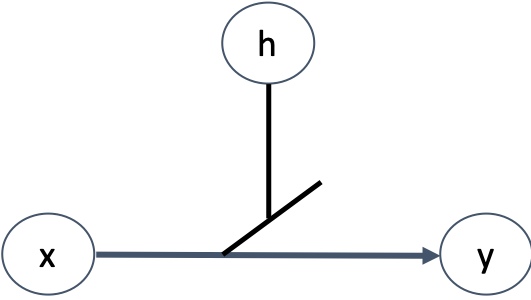
\includegraphics[scale=0.7]{fig11.png}
  \caption{Result of VAE with iteration}
  \label{fig:17-11}
\end{figure}

이번 단원에서는 예시 데이터를 이용하여 VAE를 학습한 결과를 보여줄 것이다. 28$\times$28=784차원인 MNIST 데이터를 VAE의 encoder를 이용하여 2차원으로 압축하는 것을 생각해보자. 처음에 weight는 random한 initial value를 가질 것이므로 제멋대로이다(그림 \ref{fig:17-11}의 왼쪽), iteration이 진행됨에 따라 학습이 되면 유사한 데이터에서 추출된 잠재변수끼리 군집을 이루는 듯한 형태를 보이며(그림 \ref{fig:17-11}의 오른쪽으로 점차 진행), 한 군집으로 모인 데이터 집단은 특정한 숫자를 나타내고 있을 것이다. 만약 decoder 부분이 있다면, decoder를 이용하면 재생산도 할 수 있을 것이다. 즉, 존재하지 않는 데이터에 대하여 잠재변수를 이용하여 대략적인 유추를 할 수 있을 것이다.

% 2.14 -----------------------------------------------------------------
\subsection{Variational Autoencoder for Document Modeling}
저번 단원에서는 이미지 모델링을 예시로 VAE를 사용하였다. 이번 단원에서는 VAE를 문서 모델링과 같은 discrete한 영역에서도 사용할 수 있다는 것을 보일 것이다.
\begin{equation}
	P_\theta (x_i|z) = \frac{exp\Big(-E(x_i;z,\theta) \Big)}{\sum_{j=1}^{|V|}exp\Big(-E(x_j;z,\theta) \Big)}
	\label{eq:17-14}
\end{equation}
VAE에서 decoder 부분을 수식(\ref{eq:17-14})과 같이 softmax 형태의 모델로 변환하겠다. E는 energy function인데, 수식(\ref{eq:17-15})과 같이 정의하겠다.
\begin{equation}
	E(x_i;z,\theta) = -z^TRx_i-b_{x_i}
	\label{eq:17-15}
\end{equation}
x는 one hot vector 형태의 input으로, 단어를 나타낸다. z는 잠재변수이며, 연속적인 값을 가질 것이다. z의 dimension은 clustering의 개수라고 할 수 있으며, 아마도 x와 크게 다른 dimension을 가질 것이다. 그렇다면 x와 z 사이의 관계를 정의하는 무언가가 필요할 것임을 생각할 수 있다. 이 때 두 변수 사이의 alignment를 조율하는 것이 바로 R matrix이다. 즉 R matrix란 topic z가 단어 x를 어떤 확률로 선택할 것인지에 대한 정보를 가지고 있을 것이라는 것을 알 수 있다.

결론적으로, Energy Function E란 잠재변수와 x라는 단어 사이의 관계를 학습하는 과정이다. z와 x 사이의 관계가 잘 학습되었을 경우 energy 값은 떨어지고 이것을 수식 (\ref{eq:17-14})에 적용하면 $P_\theta$가 커짐과 동일하다.       

위 설명을 통해 VAE를 sparse/discrete한 domain에도 적용할 수 있음을 알 수 있다. 다만 여기에서 문제를 제기할 수 있는 부분은, decoder만 바꿔서 불연속적인 input을 잘 해석하였다고 볼 수 있느냐는 것이다. 현재 VAE는 잠재변수 에러 부분의 확률분포로 정규분포를 사용하고 있는데, 정규분포는 연속적인 변수를 전제하는 확률분포이기 때문이다. reparameterization trick시 다른 확률분포를 이용하는 것이 추가적인 연구분야가 될 수 있을 것이다.

\begin{figure}[ht] \centering
  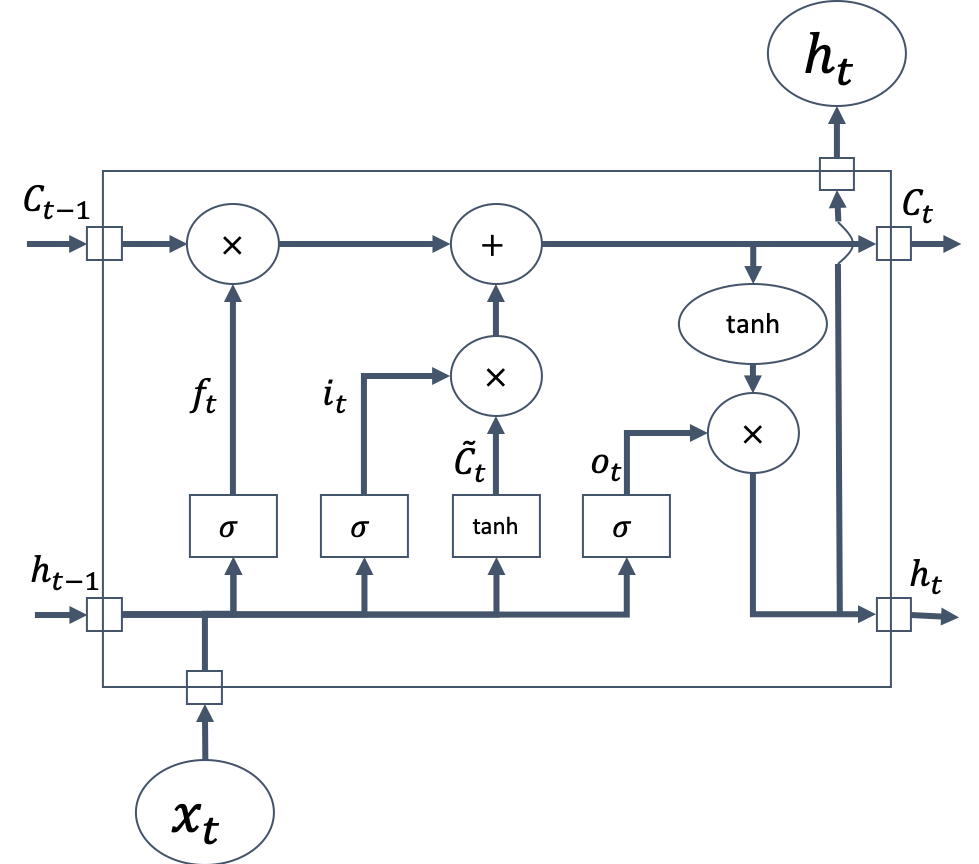
\includegraphics[scale=1.5]{fig12.png}
  \caption{Sorted list of words with association to Z in R}
  \label{fig:17-12}
\end{figure}

그림(\ref{fig:17-12})은 R matrix에서 z(가로축)에 따라 높은 값을 가지는 단어 x들을 순서대로 나열한 결과이다. 각 잠재변수 z에 대하여 높은 값을 가지는 단어들을 보면, 비슷한 주제에서 나왔을 것으로 추정되는 단어들이 같은 잠재변수에 큰 값을 가지고 있음을 알 수 있다.

% 2.15 -----------------------------------------------------------------
\subsection{Variations of Variational Autoencoder}
이번 단원에서는 VAE의 구조의 변형형태를 알아볼 것이다. 최근 VAE는 Explicit Deep Generative Model에서 가장 많은 논문들이 기반을 두고 있는 구조라고 할 수 있을 정도로 많이 다양하게 활용되고 있다. 따라서 다양한 변형형태들이 존재하는데, 수많은 변형들을 일일이 다루는 것은 의미도 없을 뿐더러 독자들에게 큰 도움이 되지 않을 것이라 생각되므로 더 기반적이고 근원적인 부분을 자극할 수 있는 변형을 다루고자 한다.
\begin{equation}
	\mathfrak{L} = -D_{KL}\Big(q_\phi(H|E)|| p_\theta(H) \Big)+\mathbb{E}_{q_\phi(H|E)}[logp_\theta(E|H)]\\
	\label{eq:17-16}
\end{equation}
\begin{equation}
	D_{KL}\Big(q_\phi(H\vert E)\Vert p_\theta(H) \Big)= -\sum_H q_\phi(H|E)log\frac{p_\theta(H)}{q_\phi(H|E)}			=\sum_H q_\phi(H|E)log\frac{q_\phi(H|E)}{p_\theta(H)}
	\label{eq:17-17}
\end{equation}
VAE의 ELBO식은 수식(\ref{eq:17-16})과 같다. 이 형태에서 무언가를 더 진행하기에는 어려워 보이므로 KL-Divergence의 형태를 바꿀 것이다.수식 (\ref{eq:17-17})에서 KL-Divergence를 확률분포 q에 대한 기댓값의 식으로 볼 수 있다. 한편, $P(E|H)P(H)=P(E,H)$이므로 E를 표현상 X로 바꿔서 다시 쓰면 결과적으로 VAE의 ELBO 식은 수식 (\ref{eq:17-18})처럼 정리된다.
\begin{equation}
	\mathfrak{L} = \mathbb{E}_{h\sim q(H|X,\phi)}[logp(x,h|\theta)-logq(h|x,\phi)] = \mathbb{E}_{h\sim q(H|X,\phi)}[log\frac{p(x,h|\theta)}{q(h|x,\phi)}]
	\label{eq:17-18}
\end{equation}
앞으로는 일전의 $p_\theta$ 확률분포와 $q_\phi$ 확률분포 인자 $\theta$와 $\phi$를 조건부의 변수로 고려하겠다. 최종적인 ELBO의 형태는 로그값의 기댓값 형태가 된다. 수식 (\ref{eq:17-18})은 ELBO의 정리된 형태이므로, 이를 경사하강법을 이용하여 최적화하는 것이 VAE를 학습하는 과정이라는 것을 독자들은 이해할 수 있을 것이다. 구체적으로, 인자 $\theta$와 $\phi$를 학습할 것이다. $\phi$와 $\theta$에 대해 미분한 것이 수식(\ref{eq:17-19})이다.
\begin{equation}
	\begin{split}
	\nabla_{\phi,\theta}\mathbb{E}_{h\sim q(H|X,\phi)}\Big[log\frac{p(x,h|\theta)}{q(h|x,\phi)} \Big]
	=\nabla_w \mathbb{E}_{h\sim q(H|X,w)}\Big[log\frac{p(x,h|w)}{q(h|x,w)} \Big] \\
	= \mathbb{E}_{\epsilon=<\epsilon_1,...,\epsilon_L>\sim N(0,I)}\Big| \nabla_wlog\frac{p(x,h(c,x,w)|w)}
	{q(h(\epsilon,x,w)|x,w)} \Big|
	\end{split}
	\label{eq:17-19}
\end{equation}
수식(\ref{eq:17-19})의 $\phi$와 $\theta$는 실질적으로 p와 q라는 확률분포를 생성하는 신경망의 weight라고 할 수 있으므로, 두 기호를 w로 표현하는 것은 충분하다. 기댓값을 구하고 그 근방에서의 최댓값을 구하는 iteration을 진행했던 EM 알고리즘에서 w 하나만 학습해도 되는 형태로 진화한 것이다. 문제는 함수 h가 너무 크게 변화한다는 것인데, 이것은 Reparameterization technique을 활용하여 해결할 수 있겠다.

% 2.16 -----------------------------------------------------------------
\subsection{Sampling Based Inference for VAE}

\begin{figure}[ht] \centering
  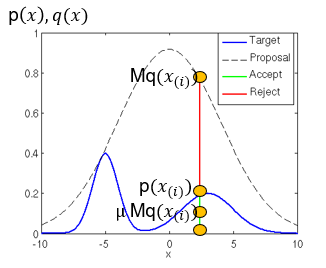
\includegraphics[scale=1]{fig13.png}
  \caption{Rejection Sampling}
  \label{fig:17-13}
\end{figure}

정리하자면 ELBO는 p 확률 분포와 q확률 분포의 비율의 로그값이다. 한편, 잘 생각해 보면 이전에 샘플기반추론(Sampling Based Inference)에서도 확률분포간의 비율을 고려했었다.

기각 샘플링(Rejection Sampling)를 떠올려보자(그림 \ref{fig:17-13}). 잘 모르는 확률분포 p에서 샘플링을 하고 싶은데, 이를 위해 잘 아는 임의의 확률분포 q를 만들고 q에 적당한 수 M을 곱하여 모든 x에 대하여 $Mq(x)\geq p(x)$를 만족하도록 했다. $\mu \sim Unif(0,1)$에 대하여 $\mu < \frac{p(x)}{Mq(x)}$이면 해당 샘플을 수용(Accept)하고, 아니면 기각(Reject)한다면, 남아있는 샘플링의 결과값은 p(x)에서 샘플링한 것과 같은 결과가 될 것이다. 이 방법의 문제는 기각되는 많은 샘플이 버려진다는 것이었다. 

한편, 중요도 샘플링(Importance Sampling)은 확률분포함수를 알아내기보다는 확률분포의 기대값이나 특정한 확률 자체를 알아내는 데에 초점을 맞추는 기법으로, 샘플이 기댓값을 정하는 데 얼마나 공헌하는 지를 알 수 있다면 기각 샘플링과 달리 샘플을 버릴 필요가 없다. ELBO 식은  기대값의 형태이므로, 기각 샘플링보다는 중요도 샘플링과 더 유사하다고 볼 수 있겠다.
\begin{equation}
	E(f) = \int f(z)p(z)dz = \int f(z)\frac {p(z)}{q(z)}q(z)dz \cong \frac{1}{L} \sum_{l=1}^L \frac{P(z^l)}{q(z^l)}f(z^l)
	\label{eq:17-20}
\end{equation}
미지의 확률분포 p를 확률 분포로 가지는 변수 z의 함수 f의 평균을 구하기 위해 중요도 가중치(Importance Weight) $\frac{p(z)}{q(z)}$를 도입하였다(수식 \ref{eq:17-20}). 이것은 확률분포 q에 의해 추출된 l개의 샘플들의 함수 f의 평균을 구하되, 중요도 가중치 $\frac{p(z^l)}{q(z^l)}$를 샘플 $z^l$의 함수값$f(z^l)$에 곱한 값들의 평균을 구하는 것과 비슷하다. 예를 들어, 함수 f가 지시함수(indicator function)라면, 수식(\ref{eq:17-21})과 같다.
\begin{equation}
	P(Z>1) = \int_{1}^{\infty}1_{z>1}p(z)dz = \int_{1}^{\infty}1_{z>1}\frac {p(z)}{q(z)}q(z)dz \cong \frac{1}{L} \sum_{l=1}^L \frac{P(z^l)}{q(z^l)} 1_{z^1>1}
	\label{eq:17-21}
\end{equation}
샘플링 방법은 샘플의 갯수, 즉 l이 커지면 커질수록 구하고자 하는 값과 유사한 값이 나올 것이다.이와 유사하게 ELBO는 $\epsilon$ 샘플링 횟수를 바꾸어서 lower bound가 더 정밀하도록 만들 수 있다.

% 2.17 -----------------------------------------------------------------
\subsection{Importance Weighted VAE}
(\ref{eq:17-18})의 ELBO에서는 $\epsilon$을 한 번 샘플링하여 VAE에 적용했었다. 만약 $\epsilon$을 여러 번(k) 샘플링한다면, ELBO를 수식(\ref{eq:17-22})와 같이 정리할 수 있다.
\begin{equation}
	\mathfrak{L} = \mathbb{E}_{\epsilon \sim N(0,1)} \Big[ log \frac{p(,h(\epsilon,x,\theta)|\theta)}{q(h(\epsilon,x,\theta)|x,\theta)} \Big]
	\label{eq:17-22}
\end{equation}

\begin{equation}
	\frac{1}{k} \sum_{i=1..k} \Big[ logw(x,h(\epsilon_i,x,\theta),\theta) \Big] = \frac{1}{k} \sum_{i=1..k} w_i
	\label{eq:17-23}
\end{equation}
p와 q의 비율을 중요도 가중치(Importance Weight) w라고 정의하면($w(x,h(\epsilon,x,\theta),\theta) = \frac{p(x,h(\epsilon,x,\theta)|\theta)}{q(h(\epsilon,x,\theta)|x,\theta)}$), w는 $\epsilon$이 바뀔 때마다 다른 값을 가질 것이다. 그러므로 w에 대해서 평균을 내볼 필요가 있다.

즉, 바뀐 ELBO는 수식 (\ref{eq:17-24})이다.
\begin{equation}
	\mathfrak{L} = \mathbb{E}_{\epsilon \sim N(0,1)} \Big[log\frac{1}{k}\sum_{i=1}^k w_i \Big]
	\label{eq:17-24}
\end{equation}
수식 (\ref{eq:17-24})은 ELBO의 부정확성을 중요도 샘플링과 연계하여 해결하였다. 이렇게 샘플링 기반 추론을 이용하여 손실함수를 가지는 구조를 Importance Weighted Autoencoder라고 한다.




\end{document}